% For more detailed article preparation guidelines, please see: http://wellcomeopenresearch.org/for-authors/article-guidelines and http://wellcomeopenresearch.org/for-authors/data-guidelines

\documentclass[10pt,a4paper,twocolumn]{article}
\usepackage{WellcomeOR_styles}

%% Packages added manually
\usepackage{float}
\usepackage{hyperref}
\usepackage{booktabs}
\usepackage{longtable}


%% Default: numerical citations
\usepackage[numbers]{natbib}
% \bibliographystyle{custom}

%% Uncomment this lines for superscript citations instead
% \usepackage[super]{natbib}

%% Uncomment these lines for author-year citations instead
% \usepackage[round]{natbib}
% \let\cite\citep

\begin{document}

\appendix
\section*{Supplementary information}
\renewcommand{\thefigure}{SI.\arabic{figure}}
\setcounter{figure}{0}
\renewcommand{\thetable}{SI.\arabic{table}} \setcounter{table}{0}


\subsection*{Weighted interval score}
\label{sec:wis}

The weighted interval score (smaller values are better) is a proper scoring rule for quantile forecasts. It converges to the continuous ranked probability score (which itself is a generalisation of the absolute error to probabilistic forecasts) for an increasing number of intervals. The score can be decomposed into a dispersion (uncertainty) component and penalties for over- and underprediction. For a single interval, the score is computed as
  $$IS_\alpha(F,y) = (u-l) + \frac{2}{\alpha} \cdot (l-y) \cdot 1(y \leq l) + \frac{2}{\alpha} \cdot (y-u) \cdot 1(y \geq u), $$
  where $1()$ is the indicator function, $y$ is the true value, and $l$ and $u$ are the $\frac{\alpha}{2}$ and $1 - \frac{\alpha}{2}$ quantiles of the predictive distribution $F$, i.e., the lower and upper bound of a single prediction interval. For a set of $K$ prediction intervals and the median $m$, the score is computed as a weighted sum,
  $$WIS = \frac{1}{K + 0.5} \cdot \left( w_0 \cdot |y - m| + \sum_{k = 1}^{K} w_k \cdot IS_{\alpha}(F, y) \right), $$
  where $w_k$ is a weight for every interval. Usually, $w_k = \frac{\alpha_k}{2}$ and $w_0 = 0.5$.

\input SI/epinow2.tex

% table 4 weeks

\begin{figure*}
\centering
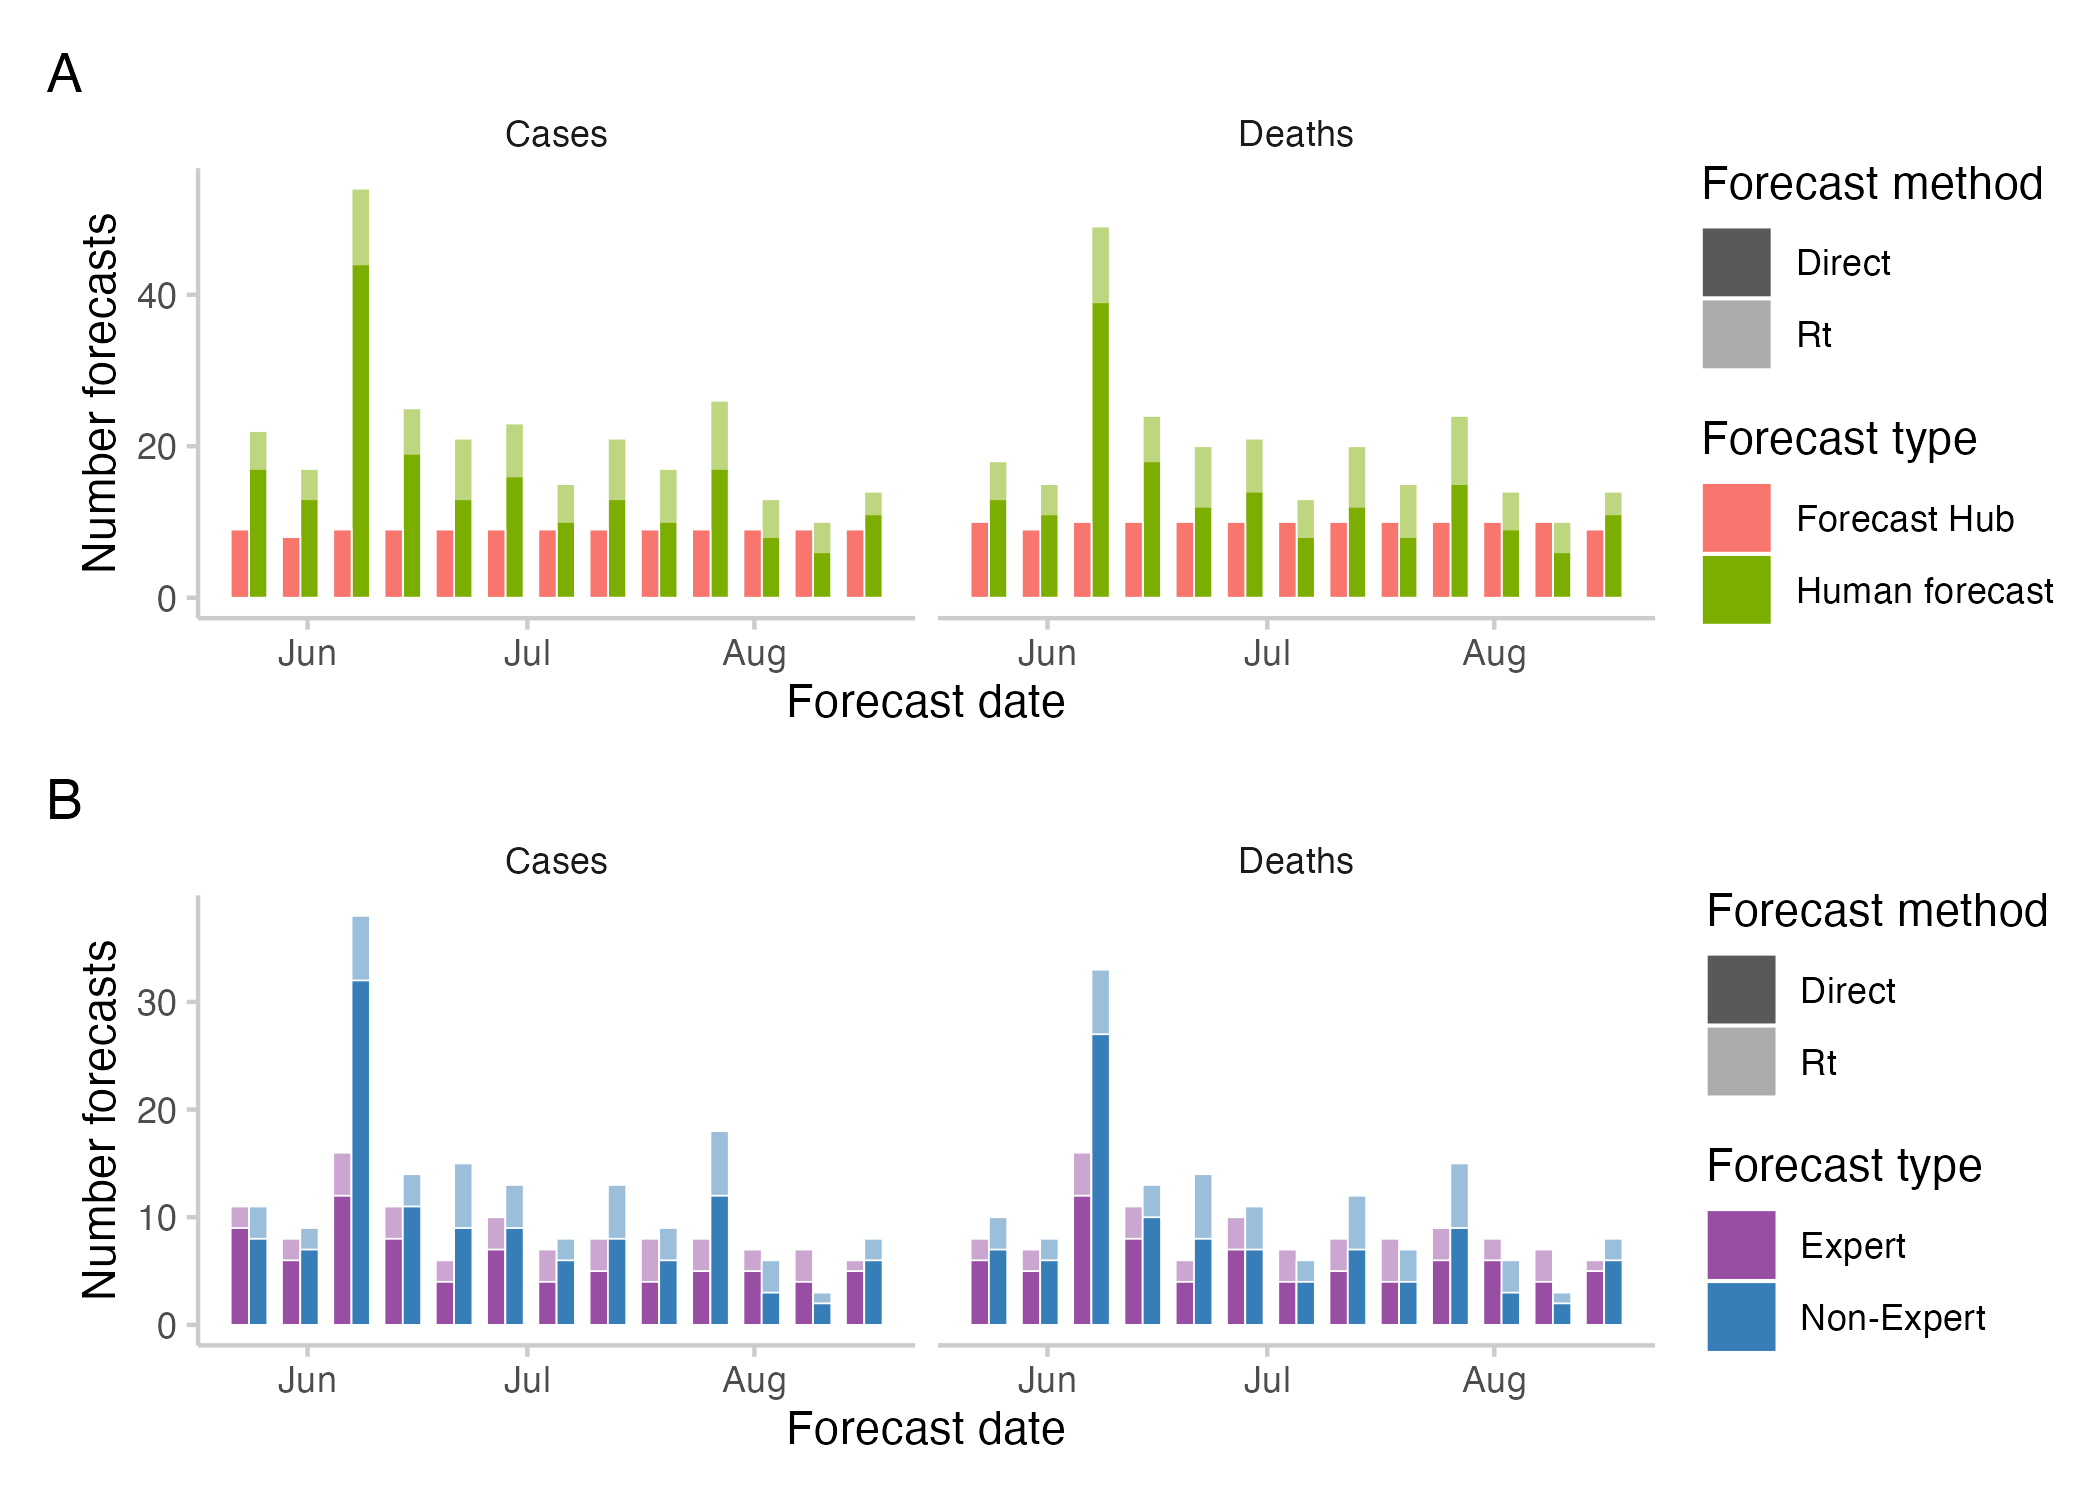
\includegraphics[width=0.99\textwidth]{../output/figures/num-forecasters.png}
\caption{\bf{Number of forecasts across the study period.} A: number of forecasts included in the Hub ensemble and the combined crowd ensemble. B: number of forecasts by "experts" and "non-experts". Expert status was determined based on the participant's answer to the question whether they "worked in infectious disease modelling or had professional experience in any related field".}
\label{fig:num-forecasters-SI}
\end{figure*}



\begin{figure*}
\centering
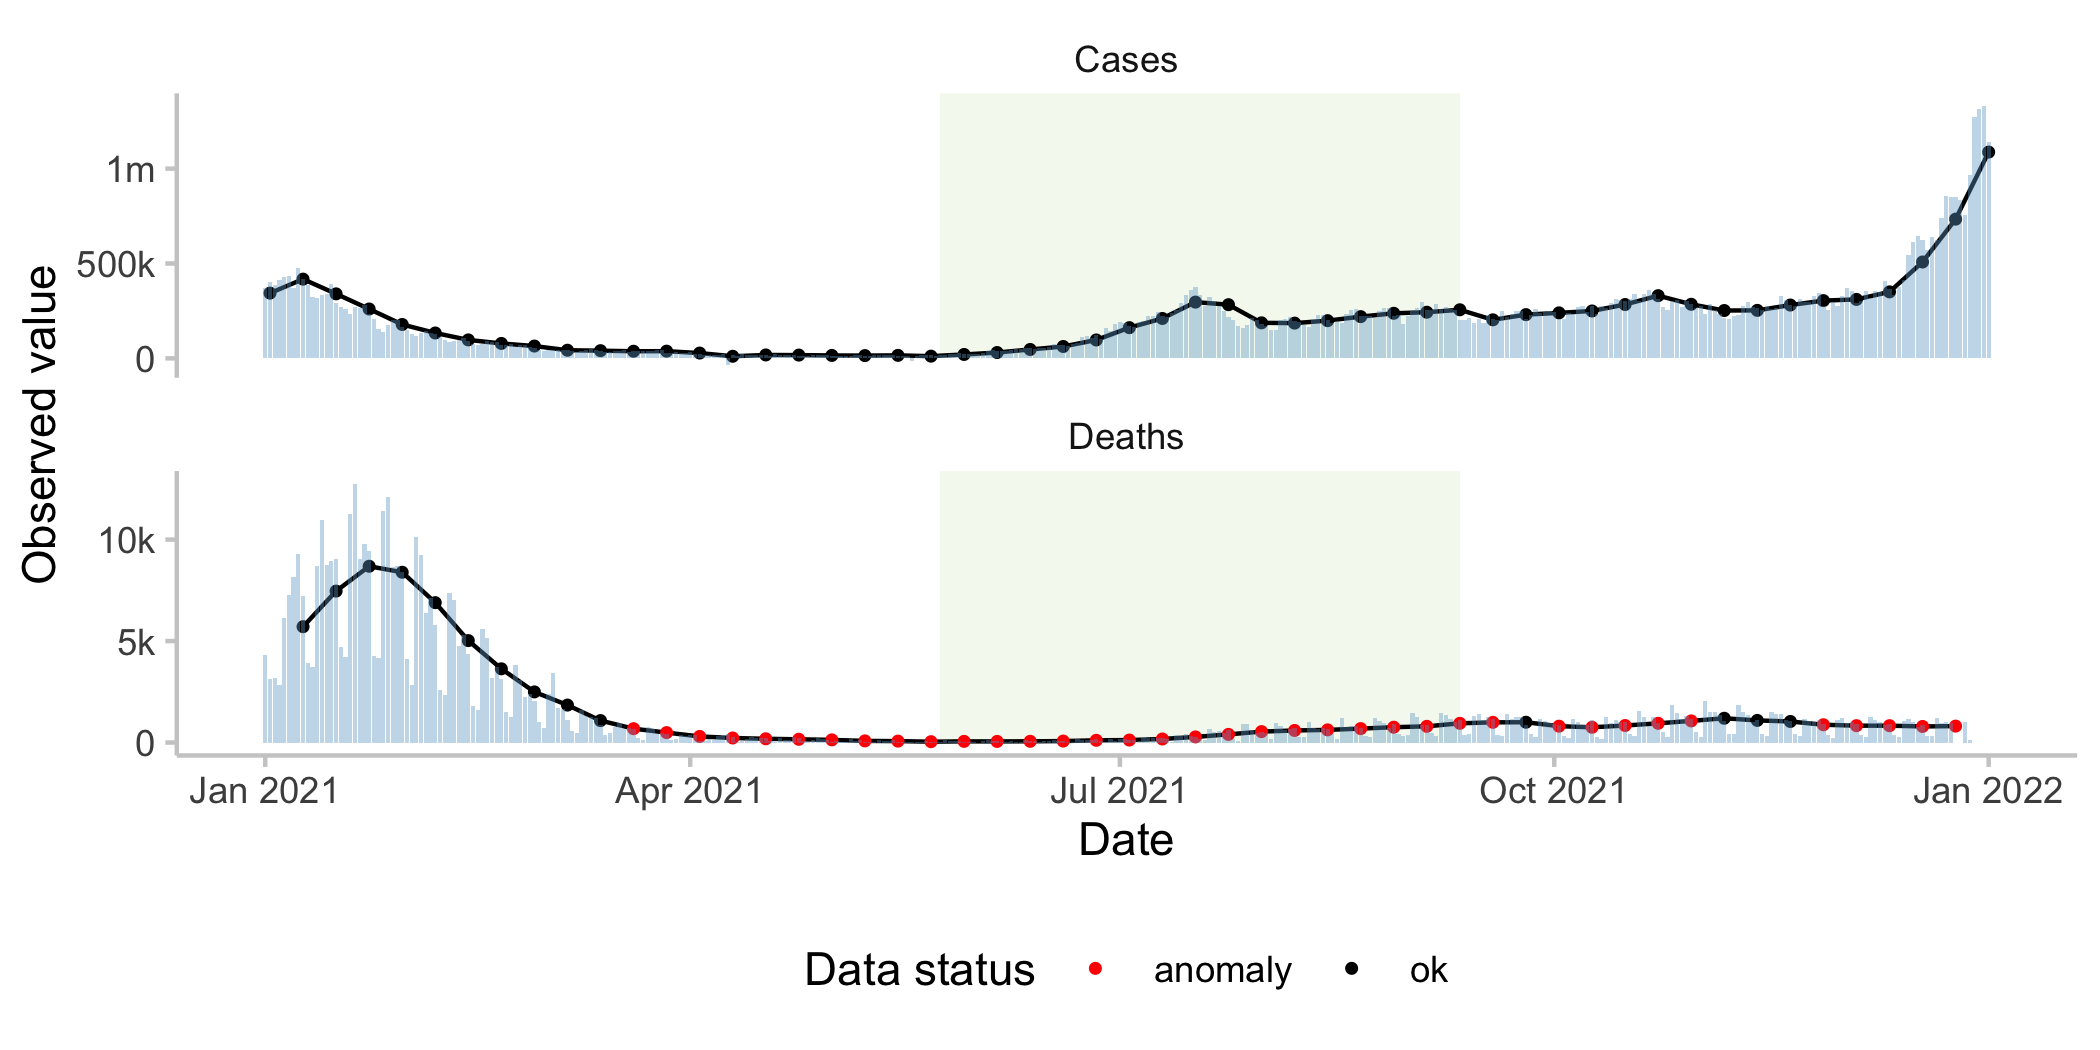
\includegraphics[width=0.99\textwidth]{../output/figures/plot-data.png}
\caption{\bf{Observed cases and deaths of COVID-19 in the UK}. A: Observed daily (bars) and weekly (black lines and points) numbers of cases and deaths as available through the European Forecast Hub when the study concluded in 2021. Daily numbers were multiplied by seven in order to appear on the same scale as weekly numbers. Red dots represent days for which the original data and the revised data disagreed by more than five percent. B: Revised data available as of February 14 2023. In August, Johns Hopkins University that provided the data switched the data stream for their death forecasts to reflect the number of death certificates that mentioned COVID-19 rather than the number of people who died within 28 days of a positive test. C: Difference between the original and revised weekly death numbers.}
\label{fig:plot-data}
\end{figure*}


\input performance-table-horizon-4.tex



\begin{figure*}
\centering
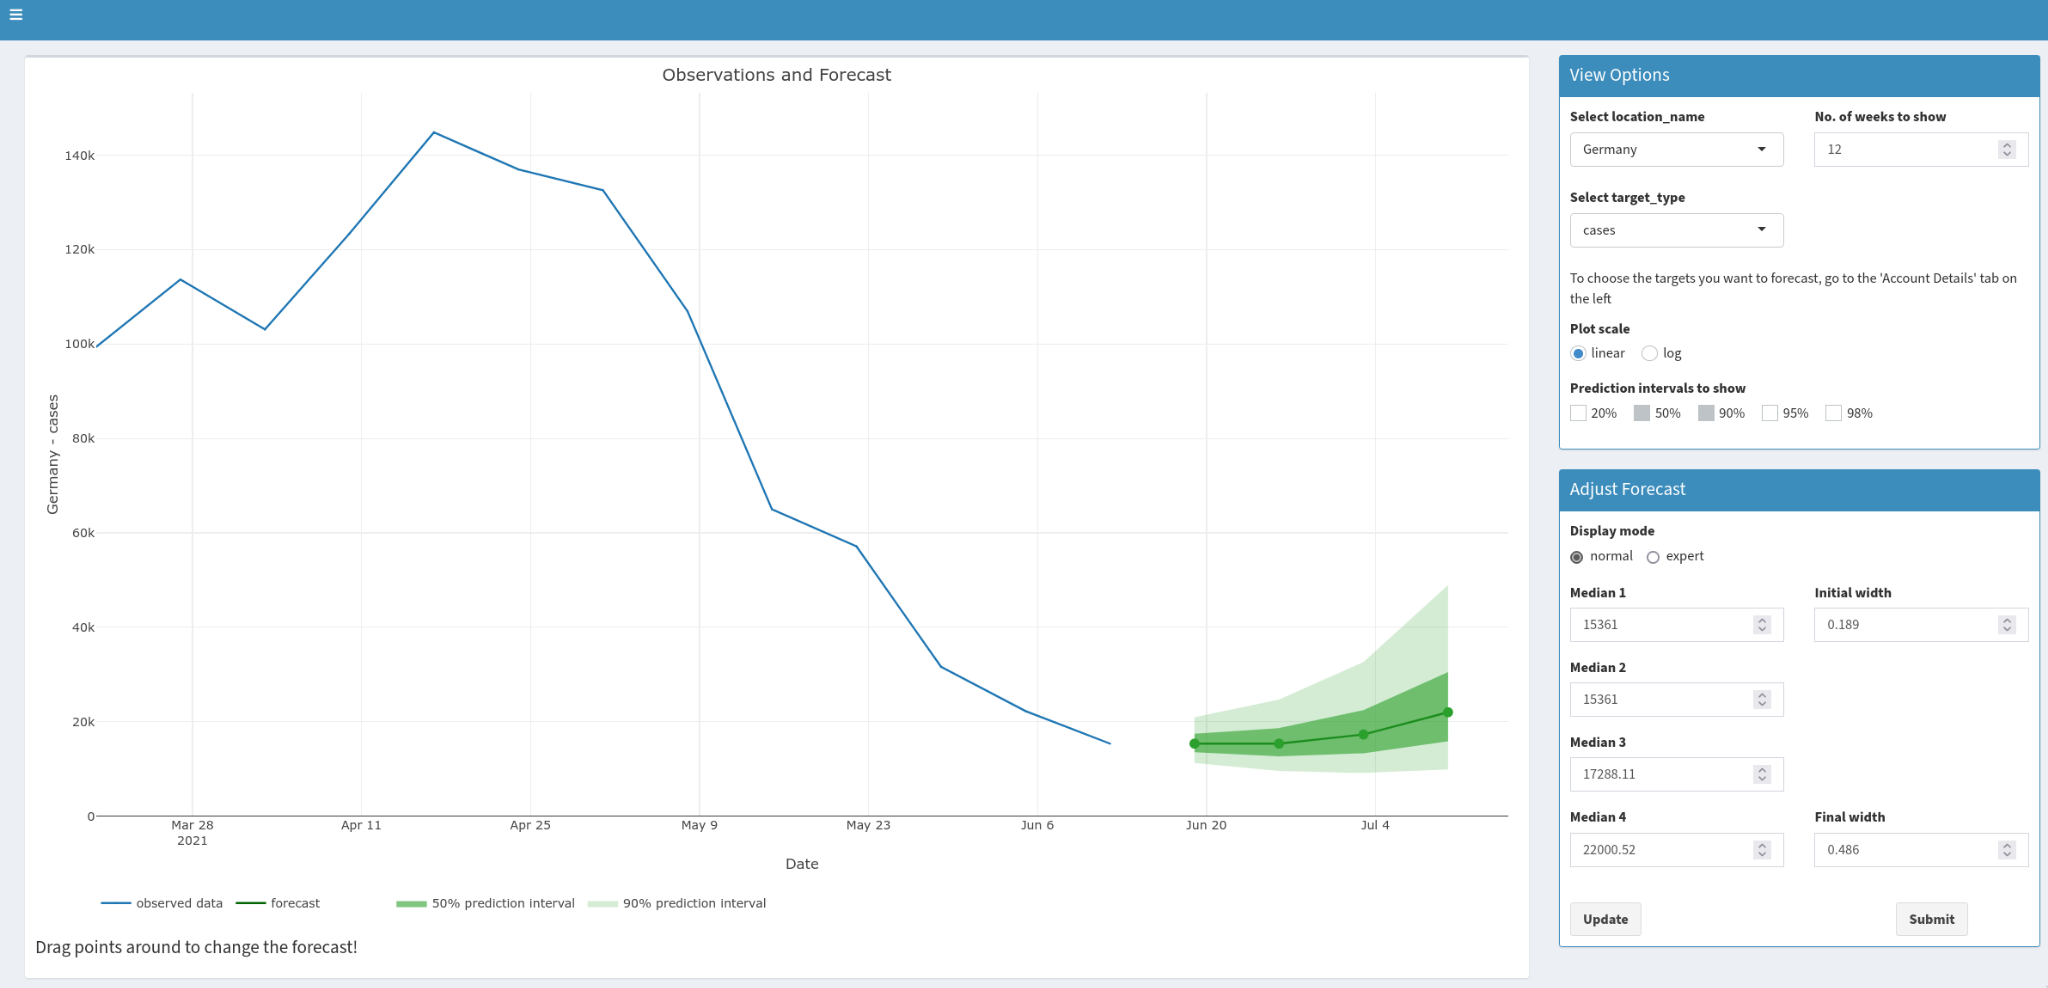
\includegraphics[width=0.99\textwidth]{../output/figures/screenshot-crowd-classical.png}
\caption{\bf{Screenshot of the direct forecasting interface.}}
\label{fig:screenshot-classical}
\end{figure*}


\begin{figure*}
\centering
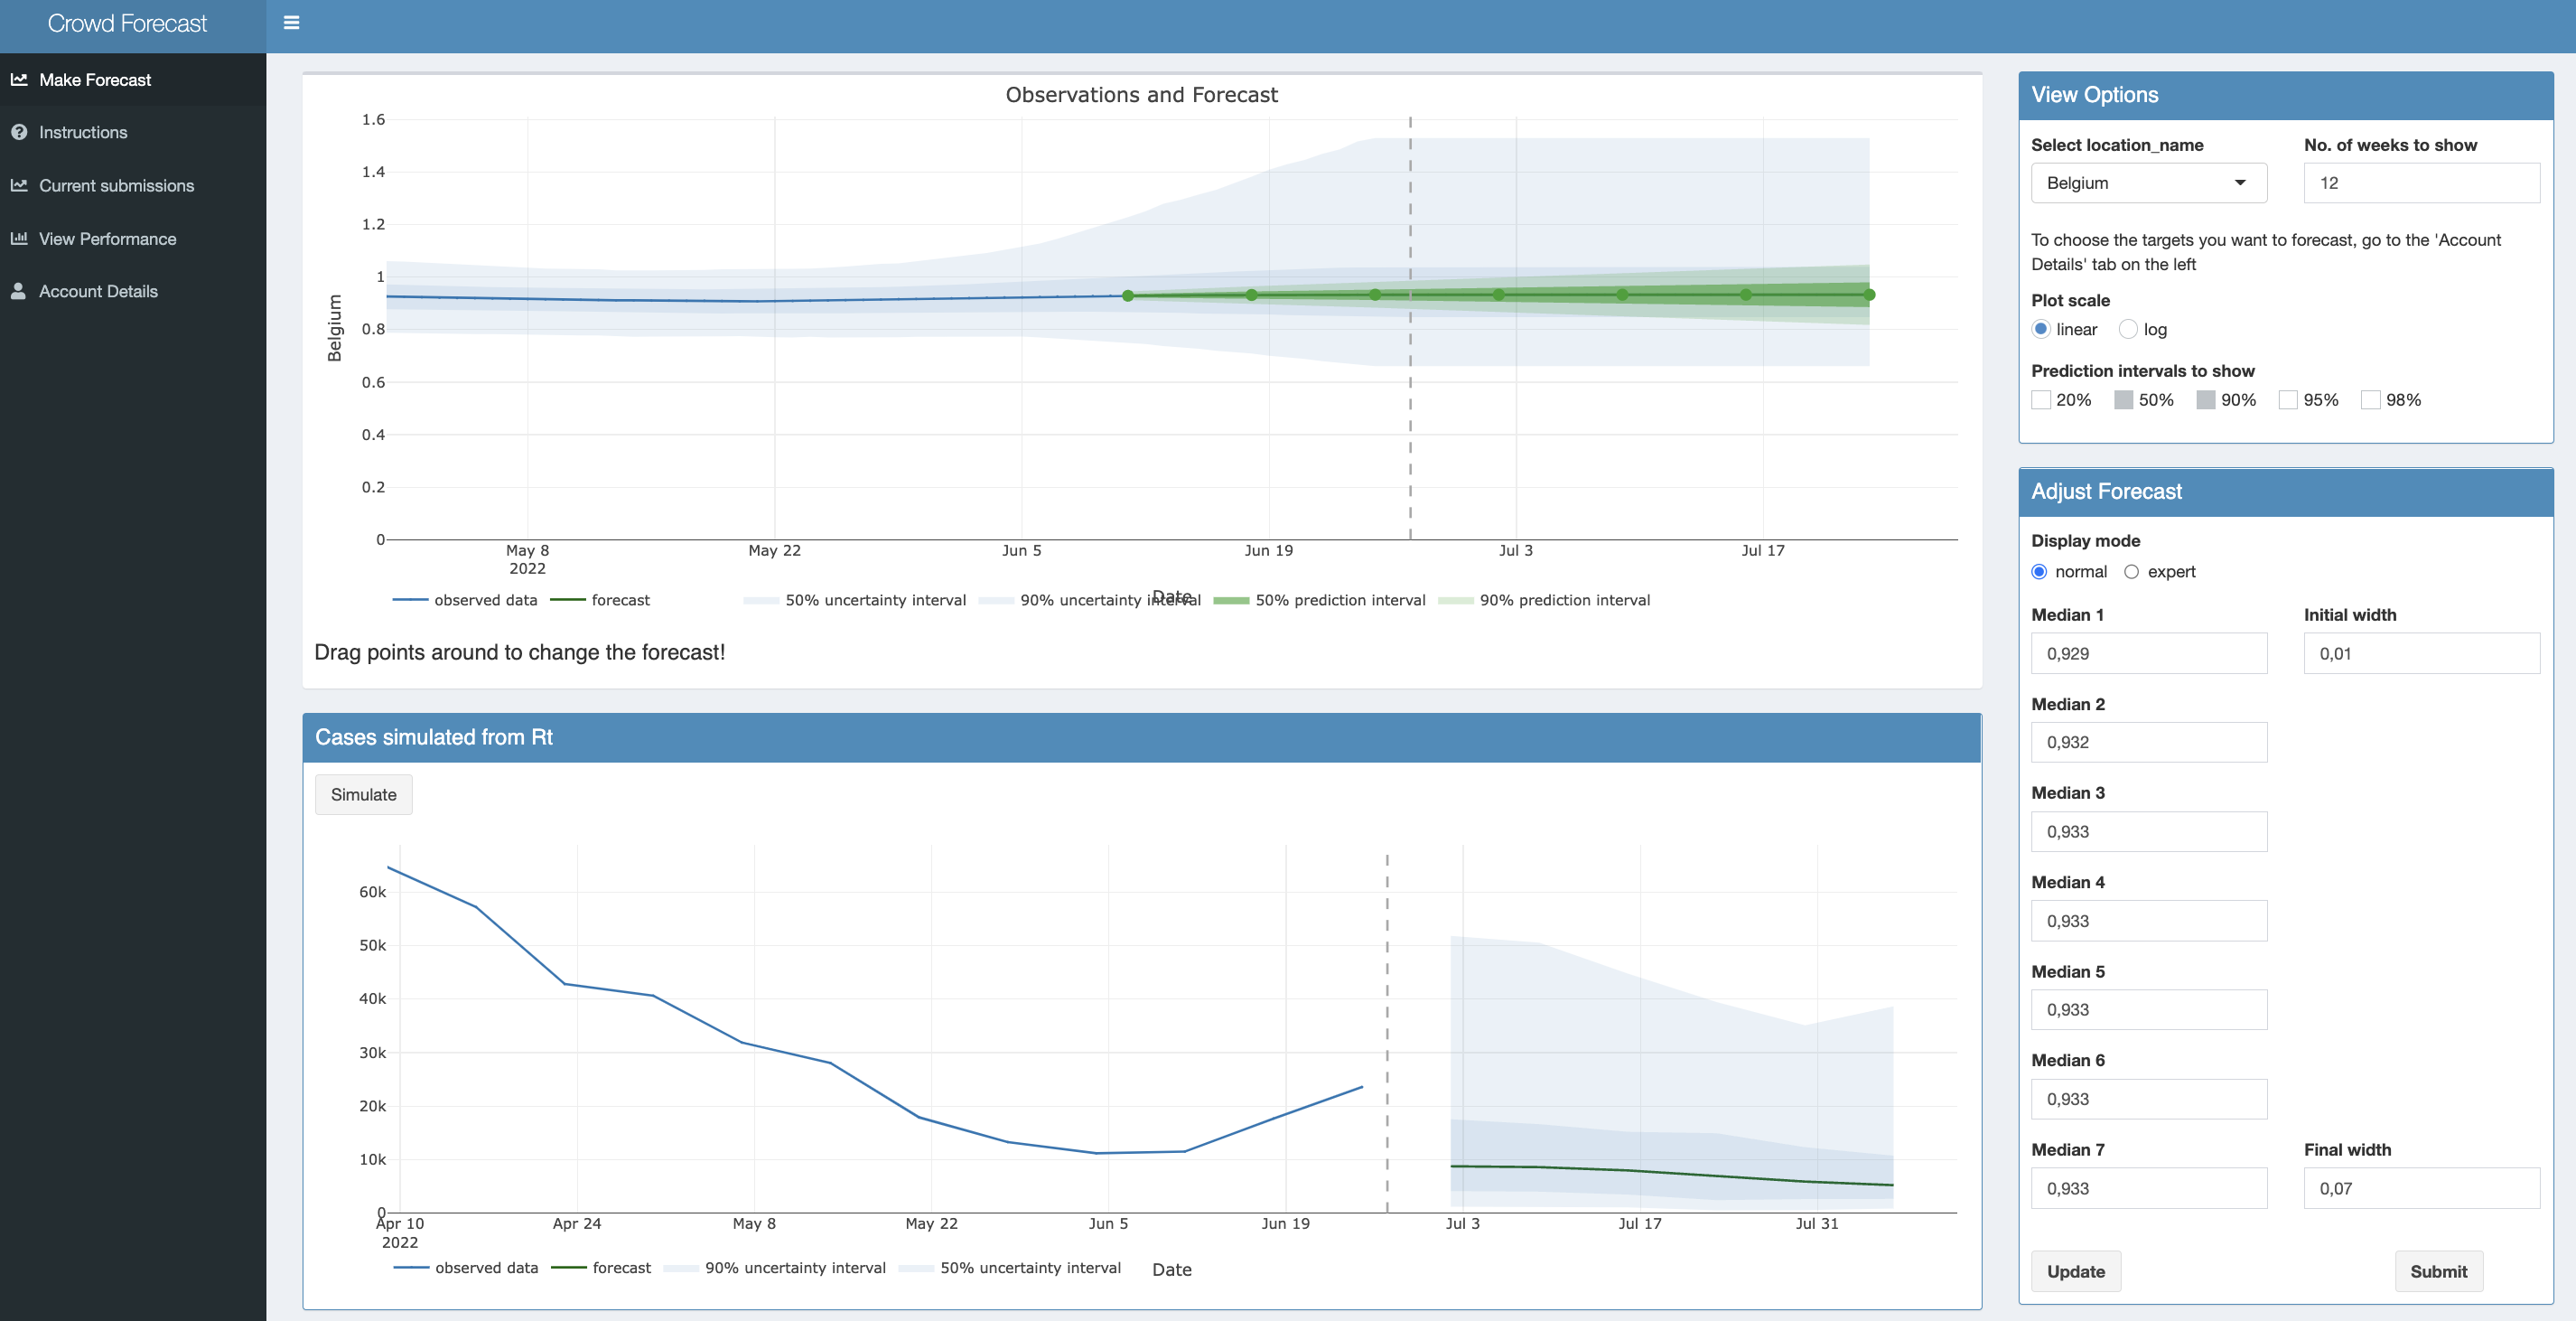
\includegraphics[width=0.99\textwidth]{../output/figures/screenshot-crowd-rt-app.png}
\caption{\bf{Screenshot of the $R_t$ forecasting interface.}}
\label{fig:screenshot-rt}
\end{figure*}



\begin{figure*}
\centering
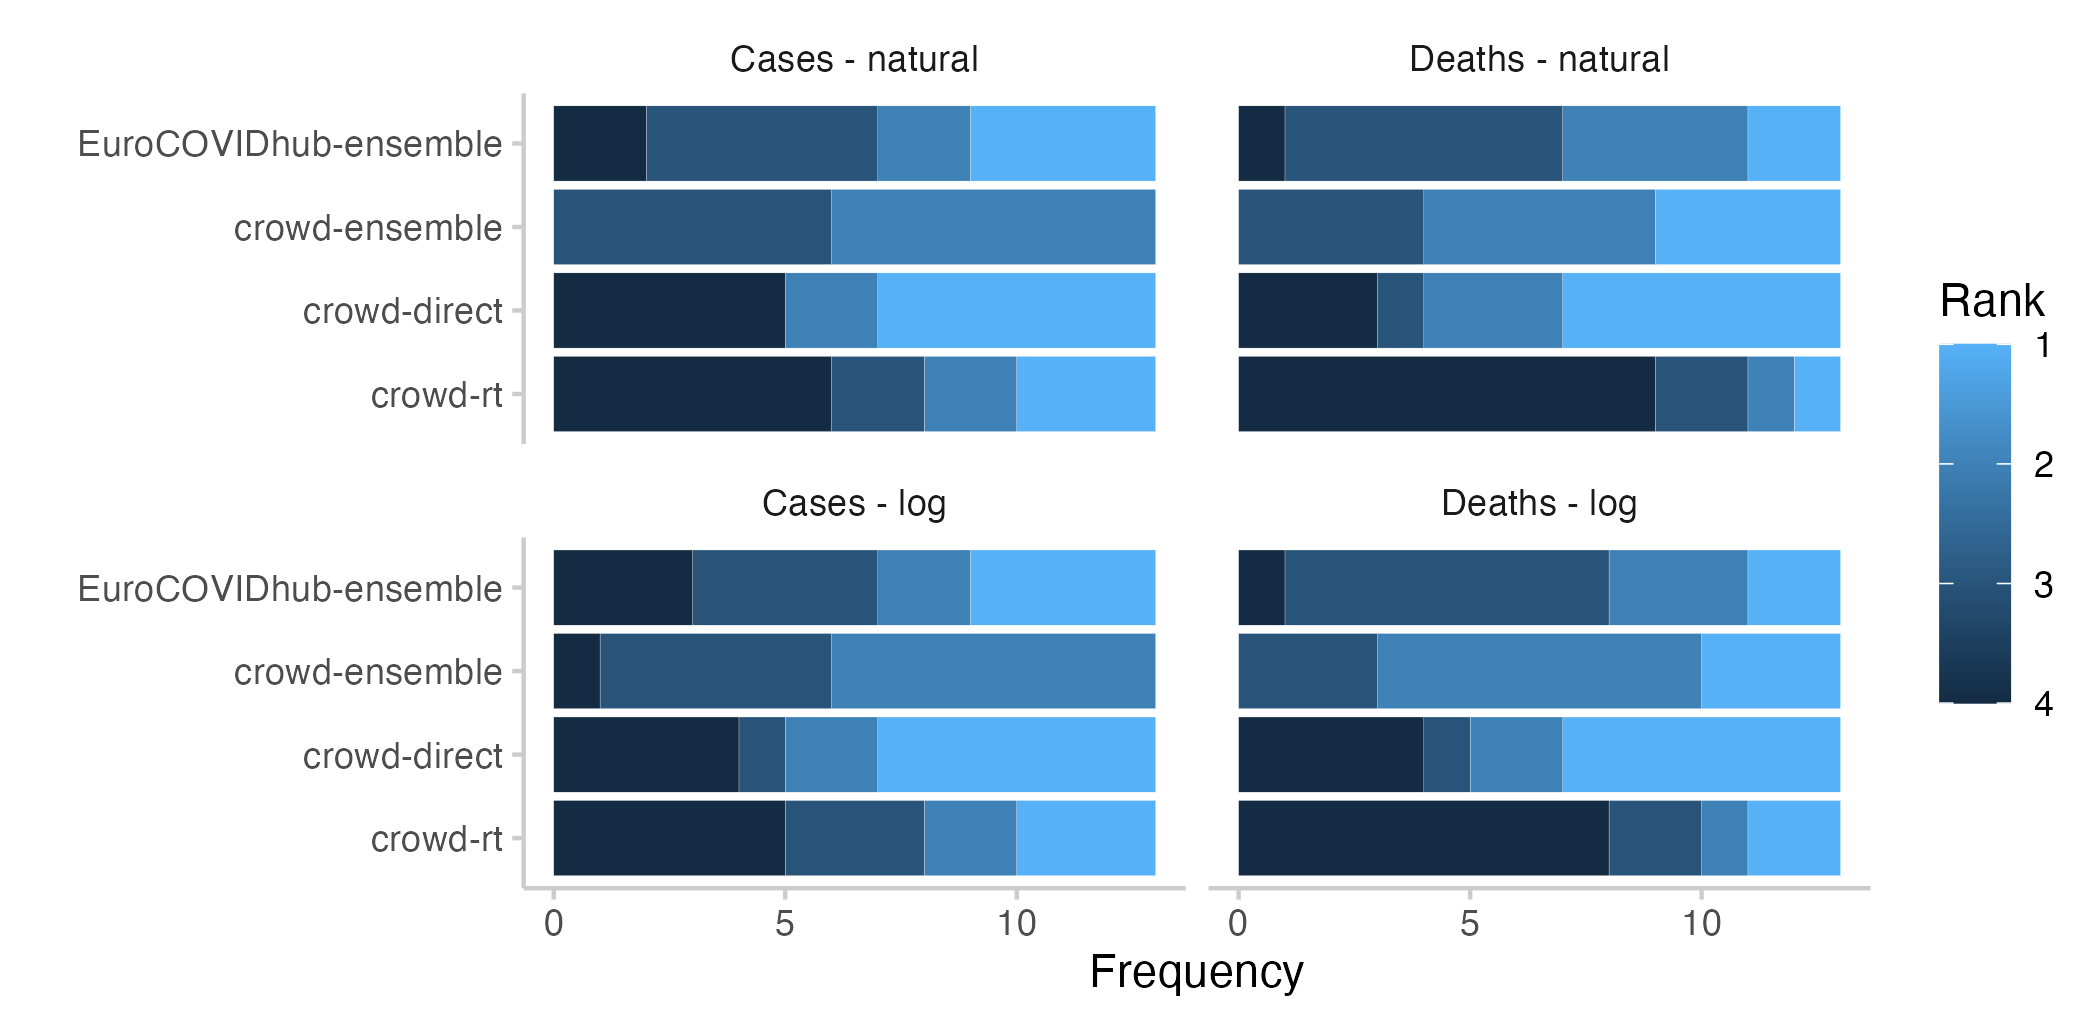
\includegraphics[width=0.99\textwidth]{../output/figures/performance-ranks-4.png}
\caption{\bf{Ranks for all forecasting approaches for four week ahead forecasts}. Colours indicate how often (out of 13 forecasts) a given approach got 1st, 2nd, 3rd, or 4th rank.}
\label{fig:performance-ranks-4}
\end{figure*}


\clearpage


\begin{figure*}
\centering
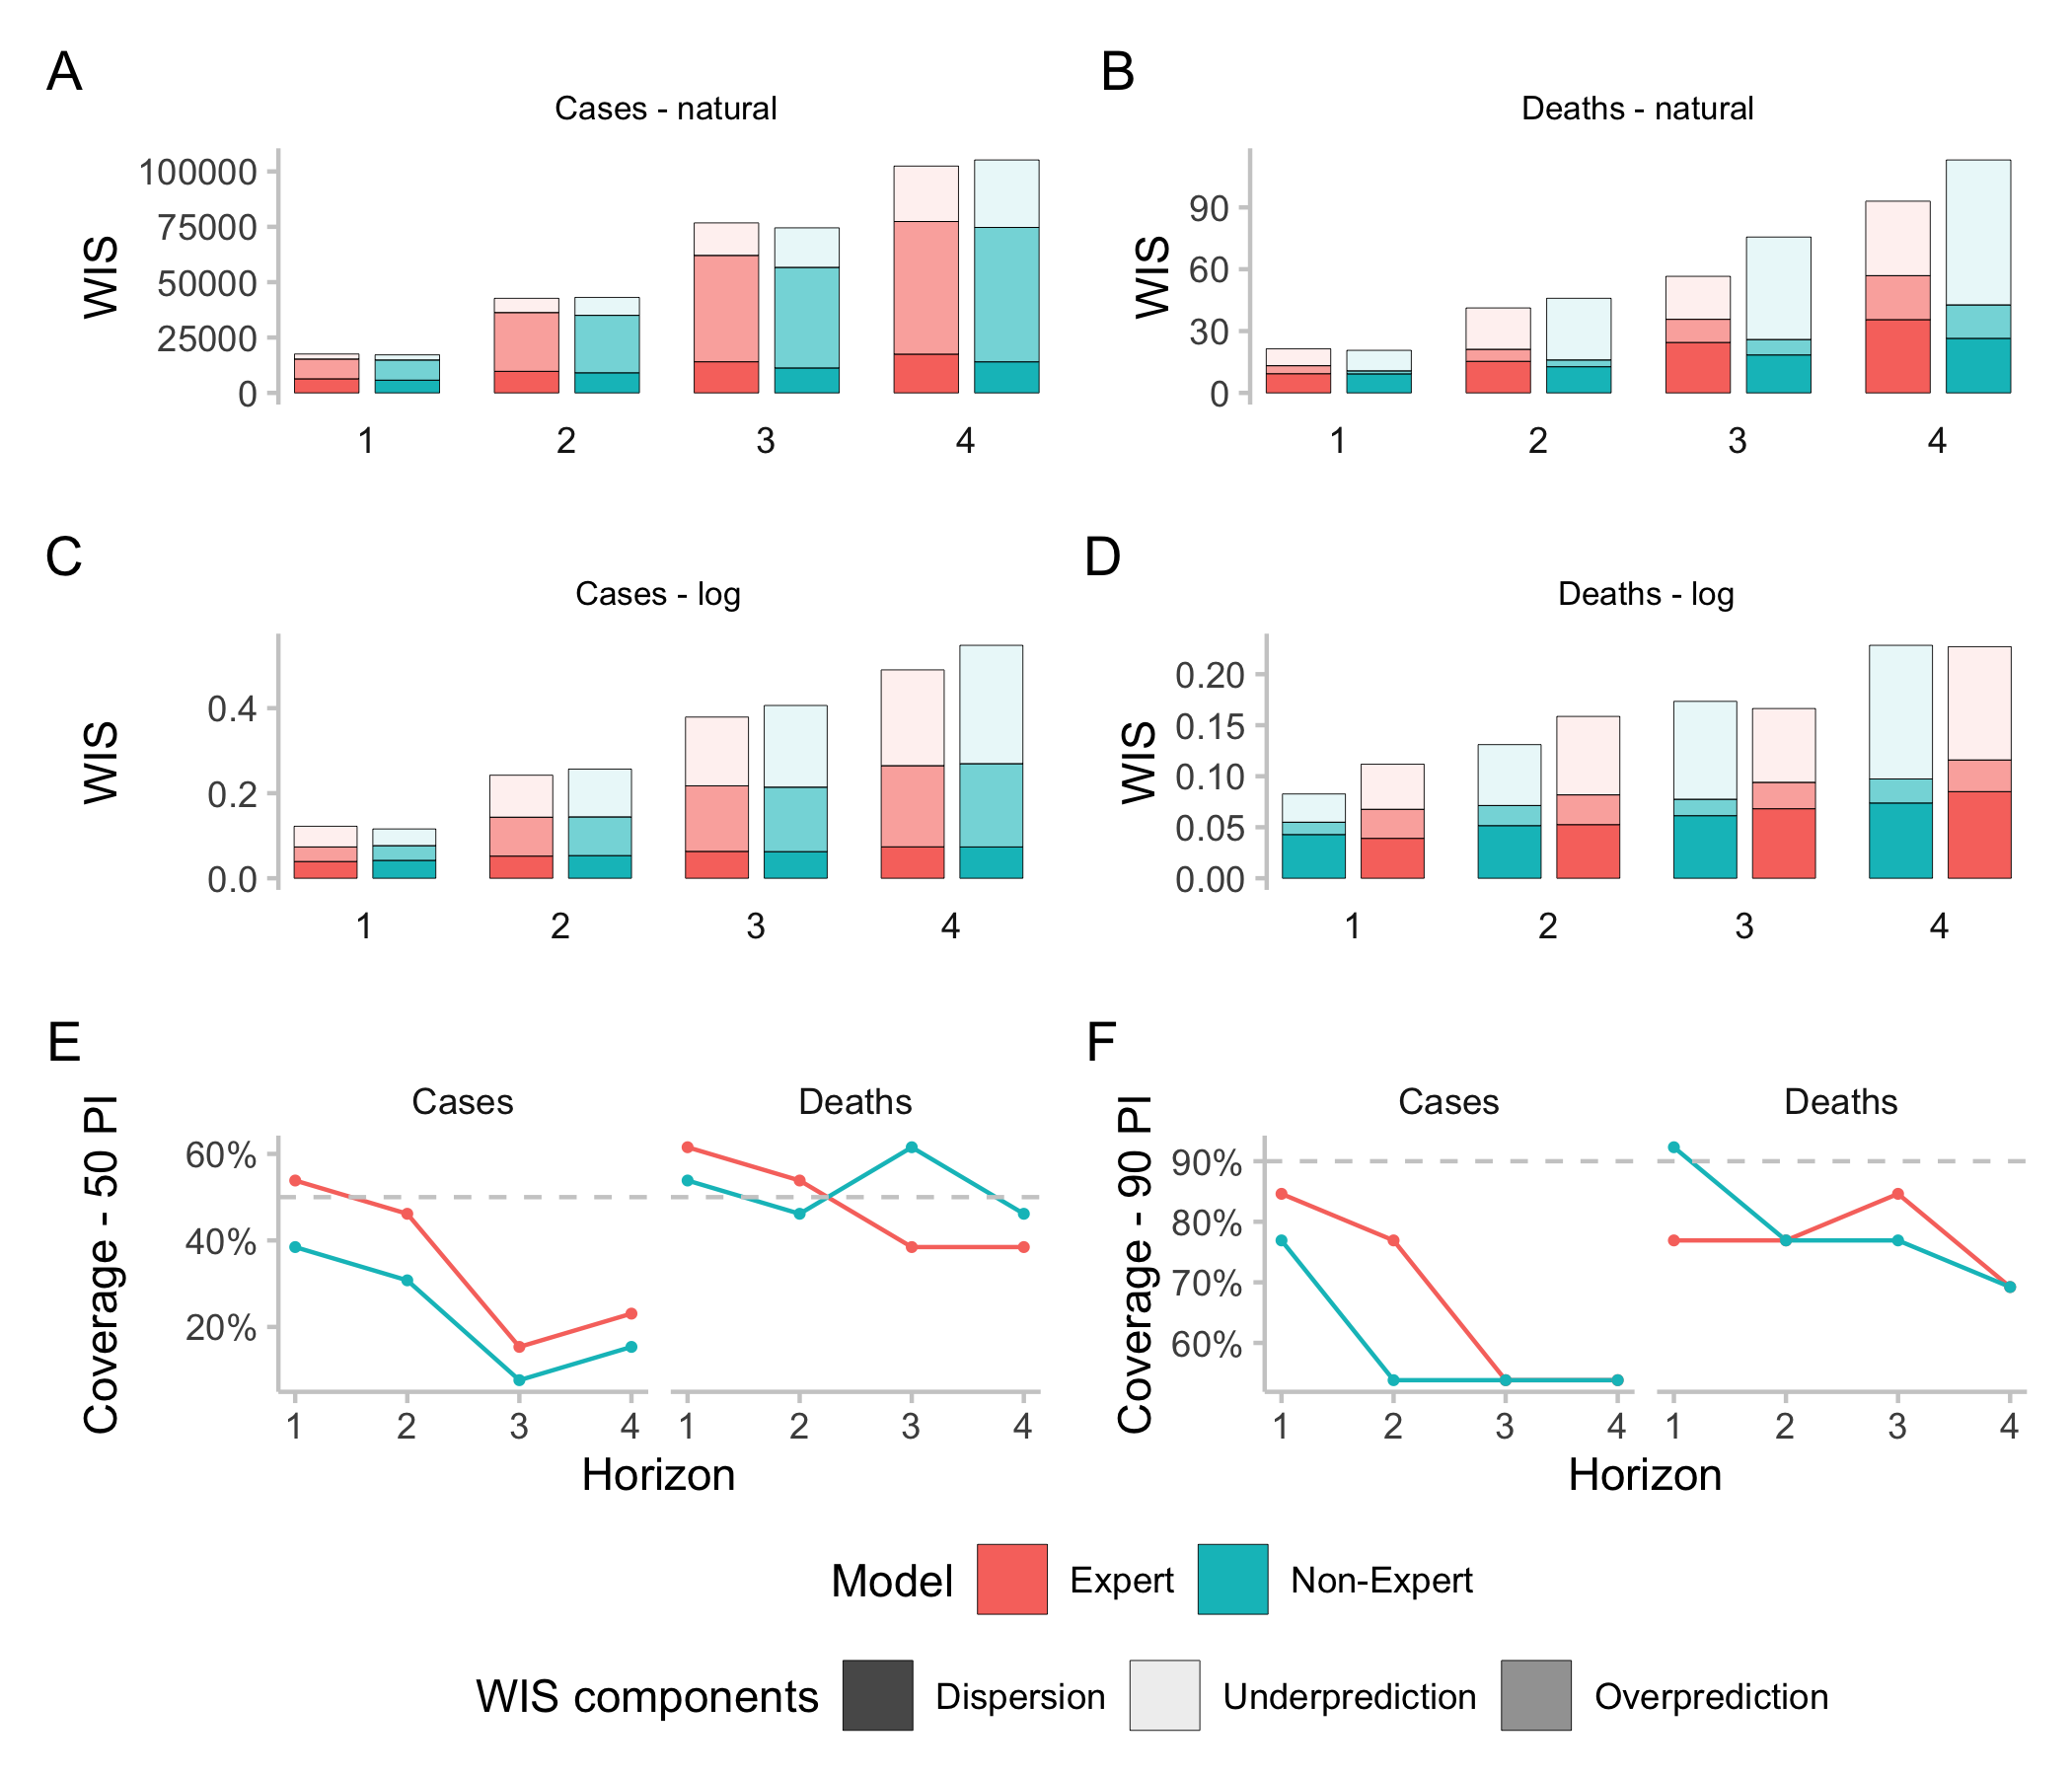
\includegraphics[width=0.99\textwidth]{../output/figures/performance-expert.png}
\caption{\bf{Predictive performance of self-reported "experts" and "non-experts" across forecast horizons.} Forecasts from "experts" and "non-experts" were combined to two separate median ensembles, including both direct and $R_t$ forecasts. A-D: WIS stratified by forecast horizon for cases and deaths on the natural and log scale. E, F: Empirical coverage of the 50\% and 90\% prediction intervals stratified by forecast horizon and target type.}
\label{fig:performance-experts-SI}
\end{figure*}


\begin{table*}[!h]

\caption{Performance for two-week-ahead forecasts of experts and non-experts. Values have been cut to three significant digits and rounded. \label{tab:scores-experts}}
\centering
\resizebox{\linewidth}{!}{
\begin{tabular}[t]{llccccllcc}
\toprule
\multicolumn{2}{c}{ } & \multicolumn{3}{c}{WIS - natural} & \multicolumn{3}{c}{WIS - log scale} & \multicolumn{2}{c}{ } \\
\cmidrule(l{3pt}r{3pt}){3-5} \cmidrule(l{3pt}r{3pt}){6-8}
Model & Target & abs. & rel. & sd & abs. & rel. & sd & Coverage 50\% & Coverage 90\%\\
\midrule
EuroCOVIDhub-ensemble & Cases & 38.2k & 1 & 55.6k & 0.25 & 1 & 0.22 & 0.38 & 0.69\\
 & Cases & 42.7k & 1.12 & 74.9k & 0.24 & 0.98 & 0.28 & 0.46 & 0.77\\
 & Cases & 43.1k & 1.13 & 67k & 0.26 & 1.04 & 0.25 & 0.31 & 0.54\\
EuroCOVIDhub-ensemble & Deaths & 37.9 & 1 & 26.9 & 0.13 & 1 & 0.04 & 0.77 & 1\\
\addlinespace
 & Deaths & 41.2 & 1.09 & 41.8 & 0.16 & 1.25 & 0.15 & 0.54 & 0.77\\
 & Deaths & 45.9 & 1.21 & 56.8 & 0.13 & 1.03 & 0.08 & 0.46 & 0.77\\
\bottomrule
\end{tabular}}
\end{table*}

\begin{table*}[!h]

\caption{Performance for four-week-ahead forecasts of experts and non-experts. Values have been cut to three significant digits and rounded. \label{tab:scores-experts-4}}
\centering
\resizebox{\linewidth}{!}{
\begin{tabular}[t]{llccccllcc}
\toprule
\multicolumn{2}{c}{ } & \multicolumn{3}{c}{WIS - natural} & \multicolumn{3}{c}{WIS - log scale} & \multicolumn{2}{c}{ } \\
\cmidrule(l{3pt}r{3pt}){3-5} \cmidrule(l{3pt}r{3pt}){6-8}
Model & Target & abs. & rel. & sd & abs. & rel. & sd & Coverage 50\% & Coverage 90\%\\
\midrule
EuroCOVIDhub-ensemble & Cases & 38.2k & 1 & 55.6k & 0.25 & 1 & 0.22 & 0.38 & 0.69\\
Expert & Cases & 42.7k & 1.12 & 74.9k & 0.24 & 0.98 & 0.28 & 0.46 & 0.77\\
Non-Expert & Cases & 43.1k & 1.13 & 67k & 0.26 & 1.04 & 0.25 & 0.31 & 0.54\\
\addlinespace
EuroCOVIDhub-ensemble & Deaths & 37.9 & 1 & 26.9 & 0.13 & 1 & 0.04 & 0.77 & 1\\
Expert & Deaths & 41.2 & 1.09 & 41.8 & 0.16 & 1.25 & 0.15 & 0.54 & 0.77\\
Non-Expert & Deaths & 45.9 & 1.21 & 56.8 & 0.13 & 1.03 & 0.08 & 0.46 & 0.77\\
\bottomrule
\end{tabular}}
\end{table*}


% % See this guide for more information on BibTeX:
% % http://libguides.mit.edu/content.php?pid=55482&sid=406343

% % For more author guidance please see:
% % http://wellcomeopenresearch.org/for-authors/article-guidelines

% % When all authors are happy with the paper, use the
% % ‘Submit to WELLCOME OPEN RESEARCH' button from the menu above
% % to submit directly to the open life science journal Wellcome Open Research.

% % Please note that this template results in a draft pre-submission PDF document.
% % Articles will be professionally typeset when accepted for publication.

% % We hope you find the Wellcome Open Research Overleaf template useful,
% % please let us know if you have any feedback using the help menu above.


\clearpage
{\small\bibliographystyle{unsrtnat}
\bibliography{software, uk-forecasting-challenge}}


\end{document}